\chapter{State of the Art} \label{chap:sota}

\section*{}

\minitoc \mtcskip \noindent
This chapter describes the state of the art in visual programming tools in the Internet-of-Things context, as well as decentralized methods of work distribution in flow-based architectures. \sectionintroref{sec:slr} presents a systematic literature review on the topic of visual programming tools applied to the Internet-of-Things paradigm, which aims to answer the research questions defined in \sectionintroref{sec:slr_research_questions}. \sectionintroref{sec:slr_results} contains the results of the Systematic Literature Review, as well as their categorization. \sectionintroref{sec:slr_expanded_research} contains the additional tools found in a survey and their analysis. The discussion and analysis of the tools found as well as the answering of the research questions made previously are made in \sectionintroref{sec:slr_discussion}. The Systematic Literature Review conclusions are presented in \sectionintroref{sec:slr_conclusions}. Lastly, \sectionintroref{sec:sota_decentralized} contains the state of the art of visual programming tools applied to IoT that implement a decentralized architecture.

\section{Systematic Literature Review}\label{sec:slr}

A Systematic Literature Review was made to gather information on the state of the art of visual programming applied to the Internet-of-Things paradigm. The goal of a systematic literature review is to synthesize evidence with emphasis on the quality of it~\cite{SLR_guidelines}.

\subsection{Methodology}\label{sec:methodology}

During this SLR, a specific methodology was followed to reduce bias and produce the best results~\cite{SLR_guidelines}. We started by defining the research questions to be answered as well as choosing data sources to search for publications.

\subsubsection{Research Questions}\label{sec:slr_research_questions}

To reveal the current practice, research and studies related to orchestration in the Internet-of-Things that leverage visual approaches, which enable us to find the current, and pending research challenges, we outline the following research questions (RQ):

\begin{description}
    \item[RQ1] \textit{What relevant visual programming solutions applied to IoT orchestration exist?} Internet-of-Things is a paradigm with several years, and its integration with visual programming languages makes their development easier for the end-user. The tools that integrate these two paradigms are useful and reduce the overhead of programming or prototyping IoT systems.
    \item[RQ2] \textit{What is the tier and architecture of the tools found in \textbf{RQ1}?} IoT systems can belong to one or more of tiers --- Cloud, Fog and Edge --- as well as implement a centralized or decentralized architecture. A visual programming tool applied to IoT orchestration can be used to facilitate the development of systems that operate on these tiers. Each tier and type of architecture offers vantages and disadvantages, which are essential to understand the usages and characteristics of a system.
    \item[RQ3] \textit{What was the evolution of visual programming solutions applied to IoT orchestration over the years?} To understand the field of visual programming applied to IoT, more specifically, its orchestration, it is essential to perceive its evolution.
\end{description}

Answering these questions will provide insights that can be valuable for both practitioners --- in terms of summarizing what the current practices on the usage of visual programming methodologies for IoT orchestration are --- and researchers --- showing current challenges and issues that can be further researched.

\subsubsection{Databases}\label{sec:databases}

The publications retrieved during this research were retrieved from the following databases:

\begin{itemize}
    \item IEEE
    \item ACM
    \item Scopus
\end{itemize}{}

These electronic databases contain some of the most relevant digital literature for studies in the area of Computer Science, thus being considered reliable sources of information. 

\subsubsection{Candidate Searching and Filtering}\label{sec:process}

Our systematic literature review protocol followed the inclusion and exclusion criteria detailed in \tableref{tab:incexclude} and is outlined in \figureref{fig:slrpipeline}.

\begin{table}[ht]
    \centering
    \label{tab:incexclude}
    \begin{tabular}{@{} l l p{13cm} @{}}
    \toprule
    \textbf{I/E}    & \textbf{ID}  & \textbf{Criterion}                                                                                                           \\ \midrule
    \multirow{5}{*}{\rotatebox[origin=c]{90}{Exclusion}} 
       & EC1 & Not written in English. \\
       & EC2 & Presents just ideas, tutorials, integration experimentation, magazine publications, interviews or discussion papers. \\
       & EC3 & Presents a tool, framework or approach that does not support the orchestration of multiple devices. \\
       & EC4 & Has less than two (non-self) citations when more than five years old. \\
       & EC5 & Duplicated articles. \\
       & EC6 & Articles in a format other than camera-ready (PDF).
       \\ \midrule
       \multirow{3}{*}{\rotatebox[origin=c]{90}{Inclusion}} 
       & IC1 & Must be on the topic of visual programming in Internet-of-Things.\\
       & IC2 & Contributions, challenges and limitations are presented and discussed in detail.  \\
       & IC3 & Research findings include sufficient explanation on how the approach works.  \\
       & IC4 & Publication year in the range between 2008 and 2019. \\
       & IC5 & Is a survey that focus visual programming in IoT or 
        \\ \bottomrule
    \end{tabular}
    \caption{Inclusion and exclusion criteria.}
    \end{table}
    \begin{figure}[h]
    \centering
    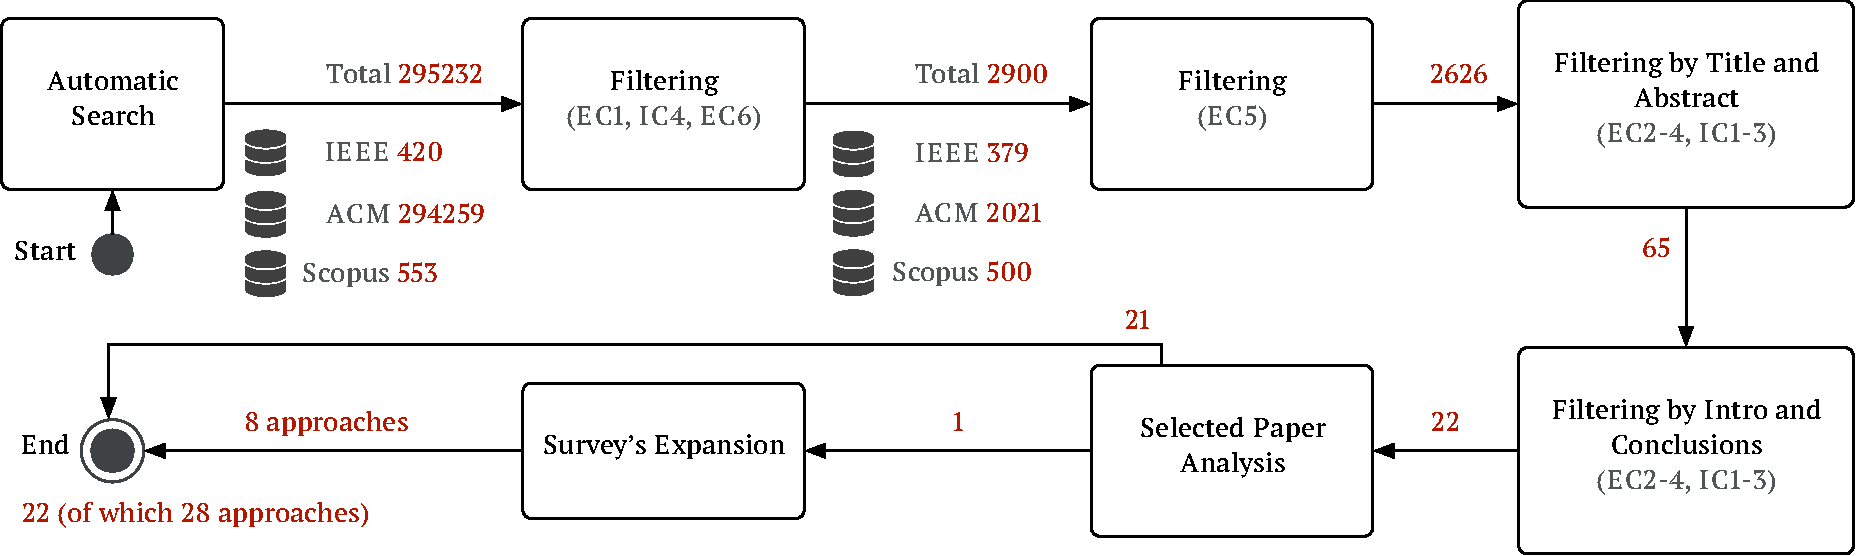
\includegraphics[width=.99\linewidth]{SLR_Pipeline.pdf}
    \caption{Pipeline overview of the SLR Protocol.}
    \label{fig:slrpipeline}
\end{figure}

We begun our search in these data sources using a query that captured the most probable keywords to appear in our target candidates, namely \emph{visual programming}, \emph{node-red}, \emph{dataflow}, and \emph{Internet-of-Things}. This led us to specify variants of the following query that are understood by the mentioned databases:
 \texttt{
((vpl OR visual programming OR visual-programming) OR (node-red OR node red OR nodered) OR (data-flow OR dataflow)) AND (IoT OR Internet-of-Things OR internet-of-things)}. This search was performed in October of 2019 and the number of results produced can be seen in the first step of \figureref{fig:slrpipeline}. 

The evaluation process of the publications then followed eight steps with specific purposes:

\begin{enumerate}
    \item \textbf{Automatic Search}: Run the query string in the different scientific databases and gather results;
    \item \textbf{Filtering} (\textit{EC1}, \textit{IC4}, and \textit{EC6}): Publications are selected regarding its (1)~language, being limited to the ones written in English language, (2)~publication date, being limited to the ones published between 2008 and 2019, and (3)~publication status, being selected only the ones that are published in their final versions (camera-ready PDF format);
    \item \textbf{Filtering to remove duplicates} (\textit{EC5}):  The selected papers are filtered to remove duplicated entries;
    \item \textbf{Filtering by \textit{Title} and \textit{Abstract}} (\textit{EC2--EC4}, and \textit{IC1--IC3}): Selected papers are revised by taking into account their \textit{Title} and \textit{Abstract}, by observing the (1)~stage of the research, only selecting papers that present approaches with sufficient explanation, some experimental results and discussion on the paper contributions, challenges and limitations, (2)~contextualization with recent literature, filtering papers that have less that two (non-self) citations when more than five years old, and (3)~leverages the use of visual notations for orchestrating and operating multi-device systems.
    \item \textbf{Filtering by \textit{Introduction} and \textit{Conclusions}} (\textit{EC2--EC4}, and \textit{IC1--IC3}): The same procedure of the previous point is followed but taking into consideration the \textit{Introduction} and \textit{Conclusion} sections of the papers;
    \item \textbf{Selected Papers Analysis}: Selected papers are grouped, and surveys are separated;  their content is analyzed in detail.
    \item \textbf{Surveys Expansion}: For the survey papers found, the enumerated solutions are analyzed and filtered taking into account their scope
    and checking if they are not duplicates of the current selected papers. 
    \item \textbf{Wrapping}: Approaches and solutions gathered from the \textit{Selected Papers Analysis} (individual papers) and from the \textit{Survey Expansion} are presented and discussed.
\end{enumerate}

The total number of publications was 2698, and, after the evaluation process, 22 publications were selected as can be seen in \figureref{fig:slrpipeline}. From those, one was a survey and the others presented approaches relevant to our research questions.

\subsection{Results}\label{sec:slr_results}

After analyzing the 22 publications, we organized them by categories; of these, one was a survey~\cite{survey_vpl_iot}, and the remaining 21 were papers describing papers that address our research questions. In that survey, the authors make an in-depth review of 13 visual programming languages in the field of IoT, comparing them using four attributes: (1)~programming environment, (2)~license, (3)~project repository and (4)~platform support. We used this survey to complement our research in \sectionref{sec:slr_expanded_research}.

The selected 21 articles described approaches that use visual programming in the IoT context having orchestration considerations. One of the tools is described in two papers, which showcases its evolution. The 20 unique solutions are:

\begin{itemize}

\begin{figure}[h]
\centering
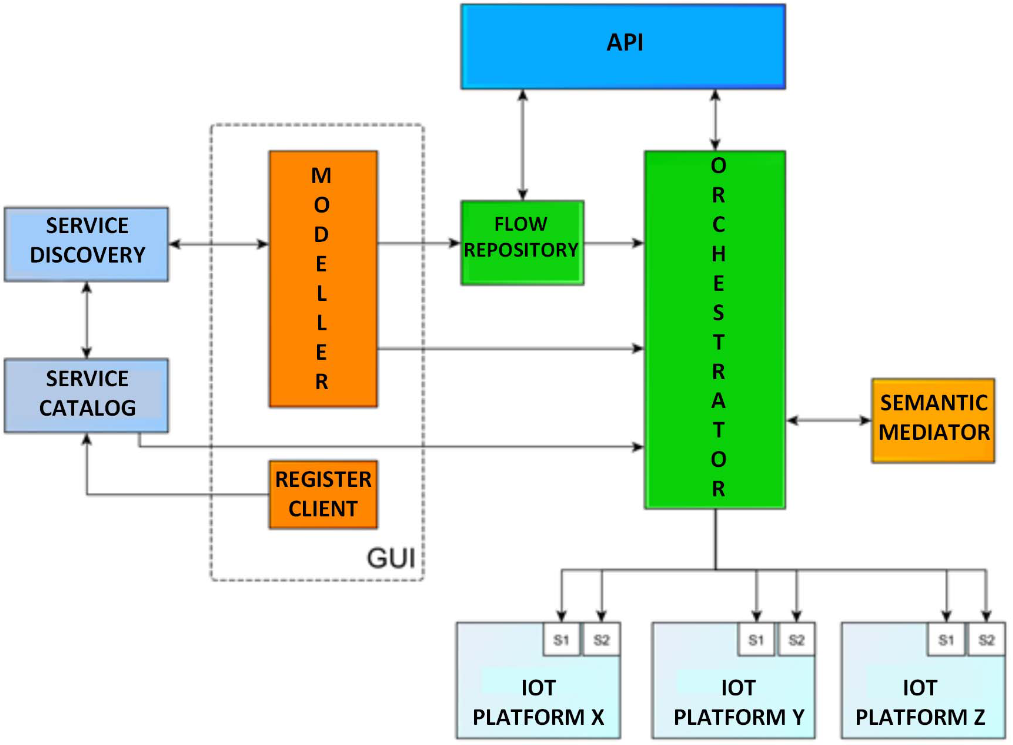
\includegraphics[width=.5\linewidth]{Belsa.PNG}
\caption[Belsa et al.~\cite{Belsa2018} solution architecture.]{Belsa et al.~\cite{Belsa2018} solution architecture. The \texttt{Modeller} is a Node-RED flow editor canvas were new flows can be created by connecting nodes that correspond to the available services (\texttt{Service Catalog and Discovery}) which are then stored in the \texttt{Flow Repository}. The \texttt{Orchestrator} is responsible managing and running the specified flows as required (by running several instances of the Node-RED runtime) and converting Node-RED calls to the different IoT Platforms \textit{native calls} (aided by the \texttt{Semantic Mediator}).}
\label{fig:belsa}
\end{figure}

\item\textbf{Belsa et al.}~\cite{Belsa2018} present a solution for connecting devices from different IoT platforms, using Flow-Based Programming with Node-RED, depicted in \figureref{fig:belsa}. Its motivation is based on the limitation imposed by the IoT platform on communication between components and extensibility, which limits the possibility to interact with other platforms' services. To validate their solution, they implemented a use case in the domain of transportation and logistics, with a service that uses five different types of applications. The developed tool offers access to available services in a centralized visual framework, where end-users can use them to build more complex applications.

\item\textbf{Ivy}~\cite{ivy} proposes the next step toward visualization applied to IoT with a visual programming tool that allows its users to link devices, inject logic, and visualize real-time data flows using immersive virtual reality. It provides the end-users with an immersive virtual reality that allows them to visualize the data flow, access to debugging tools, and real-time deployment. Each programming construct called node - data flow architecture - has a distinct shape and colour, which facilitates the understanding of the system being built or debugger for the user. The experiences made to validate the prototype were positive, with the participants being receptive to Ivy and proposing new use cases.

\item\textbf{Ghiani et al.}~\cite{personalization_of_context_dependent_apps} proposition is to build a collection of tools that allow non-developer users to customize their Web IoT applications using trigger-actions rules. The proposed solution provides a web-based tool that allows users to specify their trigger-action rules using \textit{IFTTT}, as well as a context manager middleware that can adapt to the context and events of the devices and apply rules to the system. To validate the developed tool, an example home automation application that displays sensor values and directly controls appliances were built. The results were, for the most part, positive, and the issues found are related to usability and visual clues.

\item\textbf{ViSiT}~\cite{visit} uses the jigsaw puzzle metaphor~\cite{jigsaw03} to allow its end-users to implement a system of connected IoT devices. It provides a web-based visual tool connected with a web-service that, given a jigsaw representation, generates an executable implementation. Their goal is achievable by adapting model transformations used by software developers into intuitive metaphors for non-developers to use. They validated the developed tool with a usability evaluation, which was overall positive, with a significant percentage considering the tool useful and providing real-life scenarios where they could implement it.

\item\textbf{Valsamakis and Savidis}~\cite{Valsamakis2017} propose a framework for Ambient Assisted Living (AAL) using IoT technologies, which allows for customized automation. It uses visual programming languages to facilitate their end-users - carers, family, friends, elderly - to build and modify automation. They built a visual programming framework that introduces smart objects grouping in tagged environments and real-time smart-object registration through discovery cycles. It runs on typical smartphones and tablets and is built in Javascript, allowing it to run in browsers. Their future work focuses on integrating different visual programming paradigms to accomplish the requirements of the end-user fully.

\item\textbf{WireMe}~\cite{wireme} is a solution for building, deploying, and monitoring IoT systems, built with non-developer end-users in mind but also extensible for advanced users to build over it. The developed solution makes use of Scratch, a visual programming interface, to provide its users with a customizable dashboard where they can monitor and control their IoT system as well as program automation tasks. It has a Main Control Unit responsible for communicating the device's status to the dashboard via MQTT, which is programmable using their visual interface and Lua programming language. Their tool was validated in an empirical study with students around 16 years old and engineering students without programming experience. The results were not positive, with some students not being able to create the required simple logic. Future work consists of improving programming blocks to become more intuitive.

\item\textbf{VIPLE}~\cite{viple}, Visual IoT/Robotics Programming Language Environment, is a new visual programming language and environment. It provides an introduction to topics such as computing and engineering and tools for more technical domains like software integration and service-oriented computing. It focuses on complex concepts such as robot as a service (Raas) units and Internet of Intelligent Things (IoIT) while studying the programming issues of building systems classified as such. The developed tool has been tested and used in several universities since 2015 due to its large set of features and use cases.

\item\textbf{Smart Block}~\cite{smart_block} is a block-based visual programming language and visual programming environment applied to IoT systems, that allows non-developer users to build their systems quickly. Their solution is specific to the home automation domain, like Smart Things. The language was designed using IoTa calculus, used to generalize Event-Condition-Action rules for home automation. The environment was built using a client-side Javascript library called Blockly, which allows for the creation of visual block languages. Future work for this project consists of supporting device grouping and security by expanding custom blocks, as well as extending the tool for other domains besides home automation.

\item\textbf{PWCT}~\cite{pwct} is a visual programming language applied to build IoT, Data Computing, and Cloud Computing systems. Its goal consists of reducing the cost of development of these types of systems by providing a comfortable and more productive development tool. The language was meant to compete with text-based languages such as Java and C/C++. It makes use of graphical elements to replace code. It has three main layers: (1)~the VPL layer, composed of graphical elements, (2)~the middleware layers, responsible for connecting the VPL layer to the system's view, which is the (3)~System Layer, responsible for dealing with the source code generated by the first layer. The created solution received positive feedback from the community, with more than 70,000 downloads and 93\% of user satisfaction.

\item\textbf{DDF}~\cite{ddf} is a Distributed Dataflow (DDF) programming model for IoT systems, leveraging resources across the Fog and the Cloud. They implemented a DDF framework extending Node-RED, which, by design, is a centralized framework. Their motivation comes from the possibility to develop applications from the perspective of Fog Computing, leveraging these devices for efficiency and reduced latency, since there is a significant amount of resources such as edge devices and gateways in IoT systems. They evaluated their prototype using a small scale evaluation, which was positive. The results showed that their DDF framework provides an alternative for designing and developing distributed IoT systems, despite having some open issues such as not having a distributed discovery of devices and networks.

\item\textbf{GIMLE}~\cite{gimle}, Graphical Installation Modelling Language for IoT Ecosystems, is a visual language that uses visual elements to model domain knowledge using significant ontological requirements. The goal of this language is to fill the gap of modeling requirements on the physical properties of IoT installations by proposing a new process for configuring industrial installations. It makes use of flow-based and domain-based visual programming to isolate the requirements' logical flow from their details. The developed tool supports reuse within the models, which is valuable due to the repetitive nature of industrial installations. However, it still needs to clarify its scope within the current practice and its use in production settings.

\item\textbf{DDFlow}~\cite{ddflow} is a macro-programming abstraction that aims to provide efficient means to program high quality distributed apps for IoT. The authors point to a lack of solutions for complex IoT systems programming, causing developers to build their systems, which leads to a lack of portability/extensibility and results in a lot of similar systems that do the same thing but are  ``different'' because different programmers created them. Developers use Node-Red to specify the application functionalities, and DDFlow handles scalability and deployment. The authors describe DDFlow's goal to allow developers to formulate complex applications without having to care about low-level network, hardware, and coordination details. This is done by having the DDFlow accompanying runtime dynamically scaling and mapping the resources, instead of the developer. DDFlow gives developers the possibility to inject custom code on nodes and has custom logic if the available nodes are not enough for some tasks.

\item\textbf{Kefalakis et al.}~\cite{visual_paradigm_iot_solutions_development} proposition consists of a visual environment that operates over the OpenIoT architecture and allows for the development of IoT applications with reduced programming effort. Modeling IoT services with the developed tool is made by specifying a graph that corresponds to an IoT application, which can be validated and have its code generated and performed over the OpenIoT middleware platform. It aims to fill the gap of tools that provide support for the development and deployment of integrated IoT applications. The approach taken presents several advantages: (1)~it leverages standards-based semantic model for sensor and IoT context, making it easier to be widely adopted, (2)~it is based on web-based technologies which open the possibilities of applications from developers and (3)~it is open source. 

\item\textbf{Eterovic et al.}~\cite{vpl_uml} propose an IoT visual domain-specific modeling language based on UML, with technical and non-technical users in mind. The authors defend that, with the evolving nature of IoT, the future end-user will be a non-technical person, with no programming knowledge. Attaining the issues that this can create in the future, it is crucial to create a visual language easy enough to be understood by non-technical people but expansible enough to represent complex systems. To evaluate the proposed solution, they invited 11 users of different levels of UML expertise to model a simple IoT system with the developed language. The System Usability Score was positive, as well as the Tasks Success Rate. Despite the positive score, some future actions would be the testing of the language with a more complex task as well as the integration of advanced UML notations.

\begin{figure}[h]
\centering
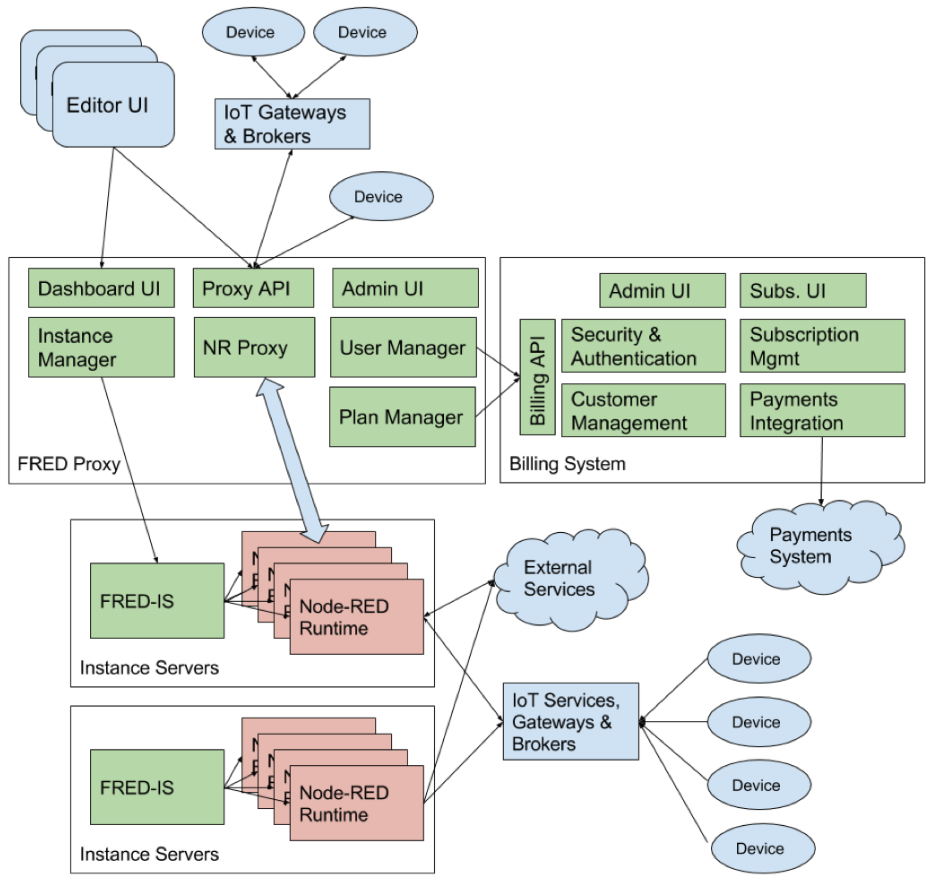
\includegraphics[width=.45\linewidth]{FRED.PNG}
\caption[FRED~\cite{fred} high-level architecture.]{FRED~\cite{fred} high-level architecture. FRED is based on Node-RED and addresses the limitation of running several flows in parallel (multiple runtimes) by orchestrating several instances of Node-RED (\texttt{FRED-IS}) using their \texttt{FRED Proxy}.}\label{fig:fred1}
\end{figure}    

\item\textbf{FRED}~\cite{fred} is a frontend for Node-RED, a development tool that makes it possible to host multiple Node-RED runtimes (\figureref{fig:fred1}). It can be used to connect devices to services in the cloud, manage communication between devices, create new web app applications, APIs and event-integrated services. To provide all these features, FRED allows the running of flows for multiple users, in which all flows get fair access to resources such as CPU, memory, storage, as well as secure access to flow editors and the flow runtime. The authors concluded that FRED is useful for users learning about Node-RED and allows users to prototype cloud-hosted applications rapidly.

\item\textbf{WoTFlow}~\cite{wotflow_dnr} is proposed as a cloud-based platform that aims to provide an execution environment for multi-user cloud environments and individual devices. It aims to take advantage of data flow programming, which allows parts of the flow to be executed in parallel in different devices. Based on this, the tool will take advantage of the ability to split and partition the flows and distribute them by edge devices and the cloud. The state of the developed tool was in the early stages, with future expansions based on the use of optimization heuristics, automatic partitioning based on calculated constraints, security, and privacy.

\item\textbf{Besari et al.}~\cite{mobile_apps_rpi,pre_mobile_apps_rpi} proposes an IoT-based GUI that aims to control sensors and actuators in an IoT system using an android application, in which the users use a visual programming language to configure and interact with the IoT system. The system was tested with a Pybot, a robot that is programmable like an IoT system, with sensors and actuators. After testing and evaluating the system, the authors came to a score of 72.917 (out of 100) for the Pybot software, which is considered ``good''. The overall acceptability of the system was "ACCEPTABLE", which led the authors to consider the application accepted by users.

\item\textbf{CharIoT}~\cite{chariot} is a programming environment that promises its end-users a solution that unifies and supports the configuration of IoT environments. It provides three blocks of support: capturing higher-level events using virtual sensors, construction of automation rules with a visual overview of the current configuration and support for sharing configuration between end-users using a recommendation mechanism. Two types of virtual sensors were developed to capture higher-level events. The programmed virtual sensor provides more accessible and understandable abstractions (defining that a room is ``cold'' if the temperature is below 20ºC). The demonstrated virtual sensors are more complex, requiring the user to provide a demonstration of the occurrence and lack of occurrence of the event (for example, the event of someone knocking on the door and the absence of someone knocking on the door). This last one requires the training of a Random Forest classifier. This programming environment is similar to IFTTT but goes one step further, with smarter event capturing and reusing of configurations, allowing the end-user to build faster and more robust IoT installations.

\item\textbf{Desolda et al.}~\cite{desolda} proposition uses a tangible programming language that allows non-programmers to configure smart objects' behaviour to create and customize smart environments. The main goal was to create, with the developed technology, a scenario of a smart museum. The authors defend that the synchronization of smart devices cannot limit the personalization of a smart environment, and it may require experts to build their narrative, much like a museum said. With this in mind, they introduced custom attributes to assign semantics to connected objects to empower and simplify the creation of event-condition-action rules. This is ongoing research focused on developing new technology with an interaction paradigm that supports the input of domain experts in the creation of smart environments. The fact that this technology uses expensive material (tabletop surface as a digital workspace) does not allow a regular user to use it, as stated in the introduction.

\item\textbf{Eun et al.}~\cite{eud_platform} proposes an End-User Development (EUD) tool that allows users to develop their applications. It uses the dataflow approach, which allows for a more generalized programming experience as well as the facility to build more complex programs with simple modules. The proposed tool has three main components: Service Template Authoring Tool, Service Template Repository, and Smartphone Application. The first one allows the end-user to build more complex methods using atomic templates (components with simple functionality, like opening a curtain if it receives a command). The Service Template Repository contains the proprietary atomic templates as well as ones built by the user. Lastly, the Smartphone Application runs and manages the applications built by the user, as well as their requirements and dependencies. The developed EUD tool was compared with \textit{IFTTT} and Zapier; other tools focused on end-user development. \textit{IFTTT} and the developed tool are similar, focusing on consumer development, IoT, and home environments, with Zapier focusing on business environments. Both Zapier and \textit{IFTTT} use the Trigger-Action paradigm (TAP), which differs from the dataflow paradigm used in this paper's tool.
\end{itemize}

The mentioned frameworks and tools were divided into the following categories, according to several characteristics:

\begin{enumerate}
    \item\textbf{Scope.} Some tools have specific use cases in mind. Therefore, knowledge of the scope of a tool is useful to assess if it solves a problem or fills a specific gap in the literature. Example values consist of \textit{Smart Cities, Home Automation, Education, Industry} or \textit{Several} if there is more than one. 
    \item\textbf{Architecture.} Visual programming tools applied to the Internet-of-Things can have a centralized or decentralized architecture, based on their use of Cloud, Fog or Edge Computing architecture. Possible values are \textit{Centralized}, \textit{Decentralized} and \textit{Mixed}.
    \item\textbf{License.} The license of software or tool is essential in terms of its usability. Normally, an open-source software reaches a bigger user base and allows them to expand and contribute to it. Possible values are the name of the tool license or N/A if it does not have one.
    \item\textbf{Tier.} IoT systems, as explained in \sectionref{sec:architectures} is composed of three tiers - \textit{Cloud}, \textit{Fog} and \textit{Edge}. A tool can interact in several of these tiers, which shapes the features it contains and how it is built.
    \item\textbf{Scalability.} Defines how the tool or framework scales. It can be calculated based on metrics used to test the performance of the system. In this case, we considered scalability in terms of number and different types of devices supported. Possible values are \textit{low}, \textit{medium}, \textit{high} or N/A, in case there is no sufficient information.
    \item\textbf{Programming.} According to Downes and Boshernitsan~\cite{vpls_survey} and also mentioned in \sectionref{sec:background_vpl}, visual programming languages can be classified in five categories: (1)~Purely Visual languages, (2)~Hybrid text and visual systems, (3)~Programming-by-example systems, (4)~Constraint-oriented systems and (5)~Form-based systems. These classifications are not mutually exclusive. It is important to know which type, so that might be possible to assess the type of experience the tool provides to the user and its architecture.
    \item\textbf{Web-based.} Defines if the visual programming language and/or environment can be used in a browser. It is useful in terms of the usability of the tool.
\end{enumerate}

\begin{table*}[h]
    \centering
    \label{tab:slr_table_results}
    \begin{threeparttable}
    \resizebox{\textwidth}{!}{
    \begin{tabular}{ l  c  c  c  c  c  c  c }
        \toprule
        \textbf{Tool} & \textbf{Scope} & \textbf{Architecture} & \textbf{License} & \textbf{Tier}  & \textbf{Scalability} & \textbf{Programming} & \textbf{Web-based}\\
        \midrule
        Belsa et al.~\cite{Belsa2018} & Several & Centralized & - & Cloud & High & Hybrid & \textbullet \\
        Ivy~\cite{ivy} & Several & Centralized & - & Cloud & Medium\tnote{7} & Purely visual &  \\
        Ghiani et al.~\cite{personalization_of_context_dependent_apps} & Home Automation & Centralized & - & Cloud & - & Form-based & \textbullet \\
        ViSiT~\cite{visit} & Several & Centralized & - & Cloud & High & Hybrids & \textbullet \\
        Valsamakis and Savidis~\cite{Valsamakis2017} & Ambient Assisted Living & Centralized & - & Cloud & - & Hybrid & \textbullet \\
        WireMe~\cite{wireme} & Education, Home Automation & Centralized & - & Cloud & - & Hybrid &  \\
        VIPLE~\cite{viple} & Education & Centralized & - & Cloud & - & Hybrid & \\
        Smart Block~\cite{smart_block} & Home Automation & Centralized & - & Cloud & - & Hybrid & \textbullet \\
        PWCT~\cite{pwct} & Several & Centralized & GNU GPL v2.0 & -\tnote{1} & High & Hybrid &  \\
        DDF~\cite{ddf} & - & Decentralized & Apache 2.0 & Fog & High & Hybrid & \textbullet \\
        GIMLE~\cite{gimle} & Industry & Centralized & - & Cloud & High & Hybrid & \textbullet \\
        DDFlow~\cite{ddflow} & Security & Decentralized & - & Fog and Edge & - & Hybrid & \textbullet \\
        Kefalakis et al.~\cite{visual_paradigm_iot_solutions_development} & - & Centralized & LGPL V3.0\tnote{3} & Cloud & - & Hybrid &  \\
        Eterovic et al.~\cite{vpl_uml} & Home Automation & -\tnote{4} & - & - & - & Hybrid & - \\
        FRED~\cite{fred} & Several & Centralized & -\tnote{5} & Cloud & High & Hybrid & \textbullet \\
        WoTFlow~\cite{wotflow_dnr} & - & Decentralized & - & Fog and Edge & - & Hybrid & \textbullet \\
        Besari et al.~\cite{pre_mobile_apps_rpi} \cite{mobile_apps_rpi} & Education & Centralized & - & Cloud & - & Hybrid &  \\
        CharIoT~\cite{chariot} & Home Automation & Centralized\tnote{6} & - & Cloud and Edge\tnote{6} & High\tnote{6} & Form-based & \textbullet \\
        Desolda et al.~\cite{desolda} & Smart Museums & - & - & - & - & Hybrid &  \\
        Eun et al.~\cite{eud_platform} & Home Automation & Centralized & - & - & - & Form-based & \textbullet \\
        \bottomrule
    \end{tabular}
    }
    \caption[Visual programming solutions applied to IoT and their characteristics.]{Visual programming solutions applied to IoT and their characteristics. Small circles (\textbullet) mean \textit{yes}, hyphens (-) means \textit{no information available}, empty means \textit{no} and asterisk (*) means more than one.}
    %\hrule width0.5\textwidth
    \begin{tablenotes}\footnotesize
        \item[1] Used for several purposes, did not specify the tier it is located in regarding IoT.
        \item[2] Since it uses Node-RED, this information was based on its architecture. 
        \item[3] Under the same license of OpenIoT.
        \item[4] No information is given regarding the architecture of the environment created, only the VPL.
        \item[5] No information about the license is given, but further research discovered that it had paid plans and no source code available.
        \item[6] CharIoT uses the Giotto stack~\cite{agarwal2016toward} from where we retrieved this information.
        \item[7] Certainty regarding this information is low. 
    \end{tablenotes}
    \end{threeparttable}
\end{table*}

\subsection{Expanded Search}\label{sec:slr_expanded_research}

The results of the Systematic Literature Review were disclosed in the previous section. However, some tools were found in a non-systematic survey~\cite{survey_vpl_iot} that are not present in the selected papers. We consider that this divergence may result from tools that have no academic publications associated with them, thus not being present in the publication databases mentioned in \sectionref{sec:databases}. One famous example is \textit{Node-RED}~\cite{node_red}. The results from the survey~\cite{survey_vpl_iot} were analyzed, the described tools were assessed against the evaluation process defined in \sectionref{sec:methodology} and characterized by the categories mentioned in \sectionref{sec:slr_results}. Using the methodology described, the results are:

\begin{itemize}

\begin{figure}[h]
\centering
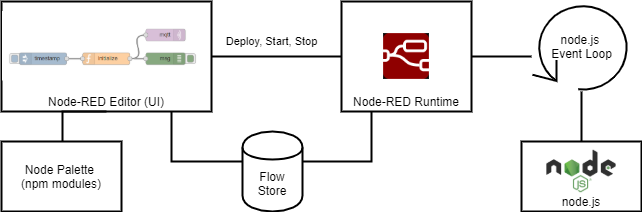
\includegraphics[width=.65\linewidth]{nodered.png}
\caption[Node-RED~\cite{node_red} high-level architecture.]{Node-RED~\cite{node_red} high-level architecture, identifying its development interface, runtime and \texttt{node.js} dependency. The \textit{flows} can be versioned and organized in projects and new modules (\emph{i.e.}, \textit{nodes}) can be added using the \texttt{node.js} dependency manager tool (\emph{i.e.}, \texttt{npm}).}
\label{fig:nodered-seq}
\end{figure}

\item\textbf{Node-RED}~\cite{node_red} is a visual programming environment applied to the IoT paradigm. It makes use of flow-based development (connecting communication and computation \textit{nodes} in \textit{flows}), supporting a wide range of devices and APIs. It has two main modules: (1) a development interface which consists of a flow drawing canvas and a \textit{node} palette, and (2) a runtime module that leverages the Node.JS event-loop to pass messages between the different \textit{nodes}~\seefigureref{fig:nodered-seq}. Due to being open-source and extendable, its large community contributes with features that enrich the tool, some of them talked about in \sectionref{sec:slr_results} (\emph{e.g.}, FRED~\cite{fred} and DDF~\cite{ddf}).

\item\textbf{NETLab Toolkit}~\cite{netlabtoolkit} is a visual environment that makes use of \textit{drag-and-drop} actions to allow users to build IoT applications. It provides a web interface to connect sensors, actuators, and others for quick prototypes.

\item\textbf{NooDL}~\cite{noodl} is a platform that provides a visual programming interface for prototyping applications. It allows for the creation of interfaces, using live data, and supporting several types of hardware. Although it is not specific to IoT, NooDL covers the programming of IoT systems. It makes use of MQTT broker agents for connecting devices and visual paradigms such as \textit{nodes}, \textit{connections}, and \textit{hierarchies} to allow the user to build its system.

\item\textbf{DGLux5}~\cite{dglux5} for DSA is a \textit{drag-and-drop} visual language and environment that allows its users to build applications tailored for Distributed Services Architecture (DSA) IoT middleware. It provides a dashboard for analyzing and controlling device data in real-time and builds the system only using visual elements.

\item\textbf{AT\&T Flow Designer}~\cite{attflowdesigner} is a visual tool incorporated in a cloud development environment, applied to the development of IoT systems. Its visual paradigm is similar to Node-RED, with the notion of \textit{nodes} and \textit{wires}. This tool provides an easy iteration and improvement of a product, as well as an easy deployment.

\item\textbf{GraspIO}~\cite{graspio} is a Graphical Smart Program for Inputs and Outputs that contains a block \textit{drag-and-drop} visual paradigm that allows its users to build applications for the \textit{Cloudio} hardware. It offers a Cloud Service that connects and manages all \textit{Cloudio} devices, making them available at the user's mobile device.

\item\textbf{Wyliodrin}~\cite{wyliodrin} is a browser-based visual programming environment that allows the development of IoT systems of several devices, such as Raspberry Pi, Arduino, Intel Galileo, Intel Edison, and others. It provides a \textit{drag-and-drop} environment, as well as support for text-based languages. A dashboard for visualizing the data collected is provided.

\item\textbf{Zenodys}~\cite{zenodys} provides a \textit{drag-and-drop} interface to build application backends as well as user interfaces. Its computing engine can run in several types of devices, from the cloud to chips, devices, and distributed computers. Zenodys contains a visual debugger as well as support for text-based programming and code generation. 
\end{itemize}

\captionsetup{belowskip=12pt,aboveskip=4pt}
\begin{table}[ht]
    \centering
    \begin{threeparttable}
    \resizebox{\textwidth}{!}{
    \begin{tabular}{ c  c  c  c  c  c  c  c }
        \toprule
        \textbf{Tool} & \textbf{Scope} & \textbf{Architecture} & \textbf{License} & \textbf{Tier}  & \textbf{Scalability} & \textbf{Programming} & \textbf{Web-based}\\
        \midrule
        Node-Red~\cite{node_red} & Several & Centralized & Apache 2.0 & Cloud and Edge & High & Hybrid text and visual system & \textbullet \\
        NETLab Toolkit~\cite{netlabtoolkit} & - & - & GNU GPL & Edge\tnote{2} & - & Hybrid text and visual system & \textbullet \\
        NooDL~\cite{noodl} & Several & - & NooDL End User License\tnote{1} & Cloud\tnote{2} & - & Hybrid text and visual system &  \\
        DGLux5~\cite{noodl} & Several & - & DGLux Engineering License & Cloud and Fog\tnote{2} & High\tnote{2} & Purely visual language &  \\
        AT\&T Flow Designer~\cite{attflowdesigner} & Several & - & GNU GPL3 & Cloud\tnote{2} & High\tnote{2} & Hybrid text and visual system & \textbullet \\
        GraspIO~\cite{graspio} & Education & - & BSD & Cloud\tnote{2} & - & Purely visual language &  \\
        Wyliodrin~\cite{wyliodrin} & Several & - & GNU GPL3 & All\tnote{2} & - & Hybrid text and visual system & \textbullet \\
        Zenodys~\cite{zenodys} & Several & - & GNU GPL3 & Cloud\tnote{2} & High\tnote{2} & Hybrid text and visual system & \textbullet \\
        \bottomrule
    \end{tabular}
    }
    \caption[Characterization of VPls applied to IoT from survey.]{Characterization of VPls applied to IoT from survey~\cite{survey_vpl_iot}. Small circles (\textbullet) mean \textit{yes}, hyphens (-) means \textit{no information available}, empty means \textit{no} and asterisk (*) means more than one.}
    \label{tab:expanded_research_results}
    \hrule width0.5\textwidth
    \begin{tablenotes}\footnotesize
        \item[1] Available at \url{https://www.noodl.net/eula}
        \item[2] Certainty regarding this information is low.
    \end{tablenotes}
    \end{threeparttable}
\end{table}{}

\subsection{Analysis and Discussion}\label{sec:slr_discussion}

The tools presented in this Systematic Literature Review passed the evaluation process defined in \sectionref{sec:process}. Tools that only supported one device were left out, as well as tools that extended a VPL applied to IoT. 

\subsubsection{Evolution Analysis}\label{sec:articles_nr_analysis}

To understand the evolution of visual programming languages applied to IoT, the publication years of the tools found in \sectionref{sec:slr_results}, as well as the launch years of the survey tools of \sectionref{sec:slr_expanded_research}, were analyzed. \figureref{fig:slr_evolution} contains the their evolution, where we can observe that there was a more substantial amount of work related to this topic in the years 2017 and 2018. The year 2019 still does not have conclusive data.

\begin{figure}[h]
\centering
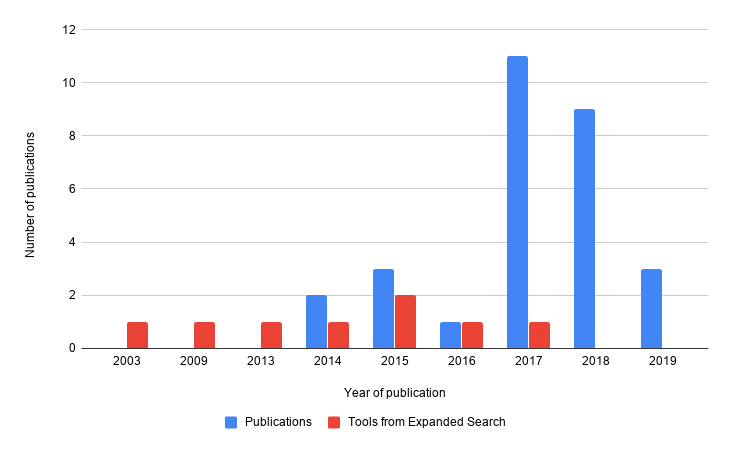
\includegraphics[width=1\textwidth]{slr_evolution.png}
\caption{Publications and tools of VPL tools applied to IoT per year.}\label{fig:slr_evolution}
\end{figure}

\subsubsection{Result Analysis}\label{sec:result_analysis}

\begin{description}
    \item [Scope] Most of the tools found have several scopes, such as education, industry or home automation. From the 28 tools, six were specific to home automation, 4 to education, 3 to specific domains, and 1 for the industry; the remainder 14 had a wide range of use cases.
    \item [Architecture] From the 28 tools found, 16 tools have a centralized architecture, three are decentralized, and the remaining nine do not present enough information to conclude on this topic.
    \item [License] Most of the tools did not mention a license and the ones who did were in its majority open-source (\emph{e.g.}, GNU GPL2, GNU GPL3, Apache 2.0 and LGPL3). 
    \item [Scalability] The majority of tools analyzed do not have scalability metrics analyzed, more specifically, the number of devices supported by them. The ones that do have high scalability, which seems to indicate that scalability is only analyzed when the tool has support for it.
    \item [Programming] From the 28 analyzed tools, 22 employ a hybrid text and visual system visual programming paradigm, while 3 use a purely visual and the other three a form-based one. 
    \item [Web-based] The majority of tools analyzed are web-based, being accessible with the use of a browser. Only one tool did not provide an environment, only a specification of a visual programming language.
\end{description}

\subsubsection{Research Questions}\label{sec:answer_slr_research_questions}

The research questions presented in \sectionref{sec:slr_research_questions} served as a way of directing the research of this Systematic Literature Review and obtain answers to relevant questions regarding the available tools that apply visual programming languages to the IoT domain. These answers are:

\begin{itemize}

\item[\textbf{RQ1}] \textit{What relevant visual programming solutions applied to IoT orchestration exist?} From the analyzed tools in Sections \ref{sec:slr_results} and \ref{sec:slr_expanded_research}, we found 28 visual programming tools applied to IoT orchestration. 

\item[\textbf{RQ2}] \textit{What is the tier and architecture of the tools found in \textbf{RQ1}?} Tables \ref{tab:slr_table_results} and \ref{tab:expanded_research_results} give an overview of the characteristics of all the tools found. In these tables and subsequent analysis in \sectionref{sec:result_analysis} it is concluded that the majority of the tools have a centralized architecture and work in the Cloud tier.

\item[\textbf{RQ3}] \textit{What was the evolution of visual programming solutions applied to IoT orchestration over the years?} As it can be observed in \sectionref{sec:articles_nr_analysis} and more specifically in \figureref{fig:slr_evolution}, there are visual programming tools applied to the orchestration of IoT since 2003, and in 2017 and 2018 there was a bigger number of publications with a focus on building these type of tools.  
\end{itemize}


\subsection{Conclusions}\label{sec:slr_conclusions}

In this Systematic Literature Review, 2698 publications were analyzed from IEEE, ACM and Scopus databases, resulting in 20 visual programming tools applied to the Internet-of-Things. A survey made on the visual programming solutions applied to IoT found during the research process resulted in 8 more tools, making a total of 28.

The results show that there is a significant number of tools that allow end-users to build IoT systems using visual programming in several different scopes. The majority of these tools have a centralized architecture and operate in the Cloud tier. Despite the considerable amount of tools, most of them do not have their source code accessible nor have a license. The results from the expanded search are more positive in this aspect, with the majority of them being open-source, such as Node-RED~\cite{node_red}, NETLab Toolkit~\cite{netlabtoolkit} and others. However, this poses a problem since there is an evident lack of open source tools.

In summary, the majority of tools found do not possess a license, employ a centralized architecture, operate in the Cloud tier and use a hybrid text and visual programming system. Thus, it propels the possibility of future research on designing and building a visual programming tool applied to IoT that is (1)~open-source, (2)~has a decentralized architecture and (3)~also operates in the Fog and/or Edge tiers.

\section{Decentralized Architectures in Visual Programming Tools applied to the Internet-of-Things paradigm}\label{sec:sota_decentralized}

Although the substantial amount of solutions found during our systematic literature (Section \ref{sec:slr_results}), only a small fraction of those aim to offer a truly decentralised solution to visual orchestration for Internet-of-Things systems. These solutions are now analysed in detail, followed by a comparison and discussion.

\subsection{DDF}\label{sec:decentralized_sota_ddf}

The work made by in WoTFlow~\cite{wotflow_dnr}, DDF~\cite{ddf} and subsequent works~\cite{fog_at_the_edge,exogenous_coordination} consists of a system built on the Node-RED framework and focused on the use case of Smart Cities. Their goal is to make a tool more suitable for the development of fog-based applications that are dependent on the context of the edge devices where they operate. 

In DDF~\cite{ddf}, the authors started by extending Node-RED and implementing D-NR (Distributed Node-RED), which contains processes that can run across devices in local networks and servers in the Cloud. The application, called flow, is built in the visual programming environment, which is running in a development server. All the other devices running D-NR subscribe to an MQTT topic that contains the status of the flow. When a flow is deployed, all devices running D-NR are notified and subsequently analyse the given flow. Based on a set of constraints, they decide which nodes they may need to deploy locally and which sub-flow (parts of a flow) must be shared with other devices. Each device has a set of characteristics, from its computational resources such as bandwidth, available storage to its location. The developer can insert constraints into the flow, by specifying which device a sub-flow must be deployed in or the computational resources needed. Further, each device must be inserted manually into the system by a technician.

\begin{figure}[h]
\centering
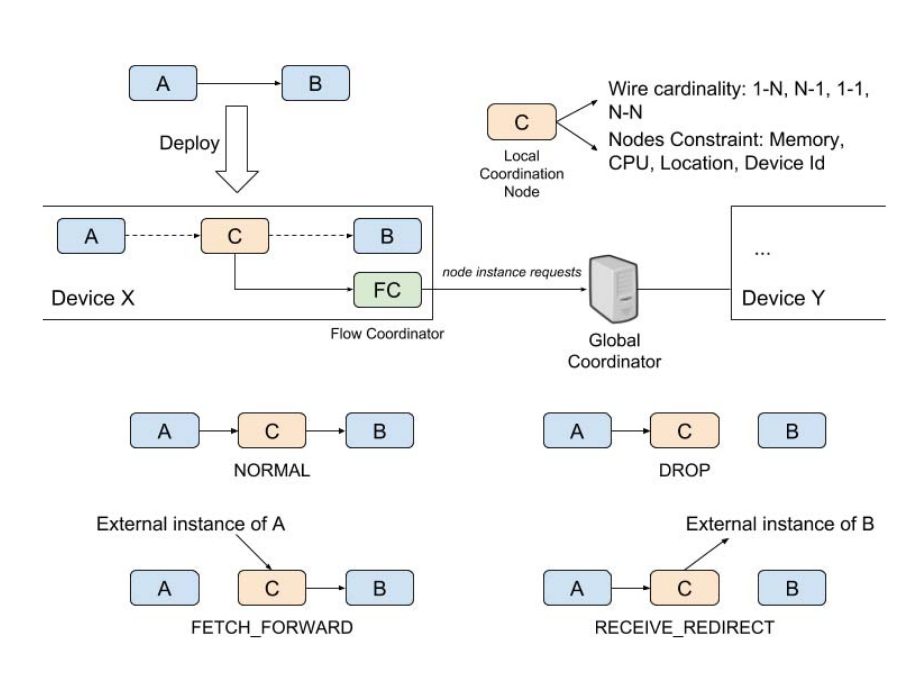
\includegraphics[width=0.8\textwidth]{dnr_exogenous_coordination.png}
\caption[Coordination between nodes in D-NR]{Coordination between nodes in D-NR\cite{fog_at_the_edge}.}\label{fig:coordination_dnr}
\end{figure}

Subsequent work to the previously mentioned tool focused on support for the Smart Cities domain. In a 2018 publication~\cite{fog_at_the_edge}, the problems addressed were the deployment of multiple instances of devices running the same sub-flow, as well as the support for more complex deployment constraints of the application flow. With this, the developer can specify requirements for each node on device identification, computing resources needed (CPU and memory) and physical location. In addition to these improvements, the coordination between nodes in the fog was tackled by introducing a coordinator node. This node is responsible for synchronising the context of the device with the one given by the centralised coordinator. In \figureref{fig:coordination_dnr} it is possible to see the four possible states of a coordinator node: (1)~NORMAL, where the node passes the data to its output, (2)~DROP, in which the node does not pass the data to other node and instead drops it, (3)~FETCH\_FORWARD, where the node gets the input from an external instance of its supposed input and (4)~RECEIVE\_REDIRECT in which the node sends the data to an external instance of its output node.

In more recent work~\cite{exogenous_coordination}, support for CPSCN (Cyber-Physical Social Computing and Networking) was implemented, making it possible to facilitate the development of large scale CPSCN applications. Additionally, to make this possible, the contextual data and application data were separated, so that the application data is only used for computation activities and the contextual data is used to coordinate the communication between those activities.

\subsection{\textit{FogFlow \& uFlow}}\label{sec:decentralized_sota_uflow}

Another approach was made in the publication by Szydlo et al.~\cite{flow_based_programming_fog}, where they focused on the transformation and decomposition of data flow. Parts of the flow can be translated into the executable parts, such as Lua code. Their contribution includes the concepts of data flow transformation, a new run-time environment called \textit{uFlow} that can be executed on a variety of resource-constrained embedded devices and the integration with the Node-RED platform. 

\begin{figure}[h]
\centering
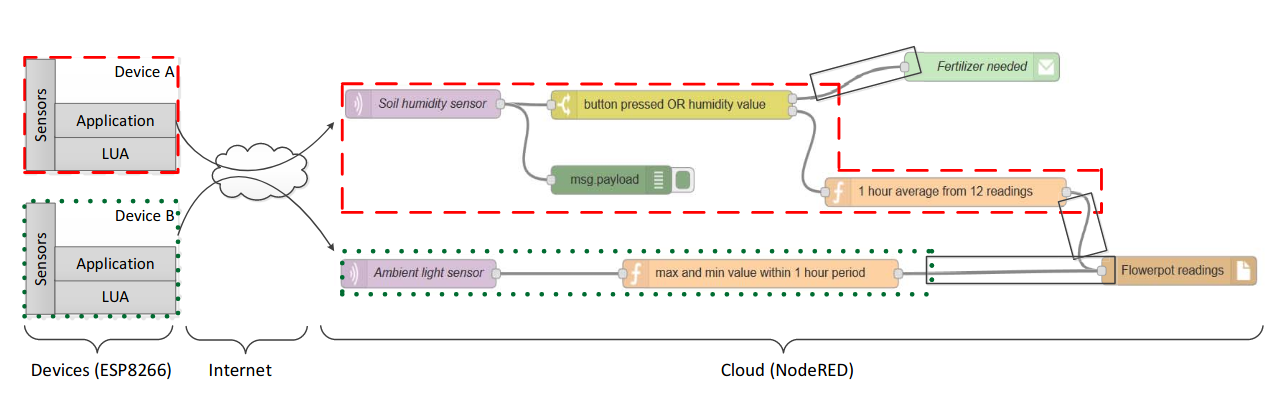
\includegraphics[width=0.9\textwidth]{uflow_1.png}
\caption[Partition and assignment of parts of the flow]{Partition and assignment of parts of the flow\cite{flow_based_programming_fog}.}\label{fig:uflow_1}
\end{figure}

The solution consisted of the transformation of a given data flow, where the developer chooses the computing operations that will be run on the devices. The operations that will run directly on the devices are implemented in the form of embedded software, using the developed framework \textit{uFlow}, which allows parts of the flow to be run on heterogeneous devices. All this is integrated with Node-RED. The communication between the devices is made only through the Cloud, with no support for peer-to-device communication. The results were promising, with a decrease in the number of measurements made by the sensors. However, there was room for improvement, with the automation of the decomposition and partitioning of the initial flow. Another improvement would be the detection bottlenecks which will move computations accordingly from the cloud to the fog.

\figureref{fig:uflow_1} represents a situation of partitioning and assignment of tasks. There are two IoT devices and a Node-RED instance running in the Cloud. The system's goal is to measure soil humidity and ambient light. If a button is pressed or fertiliser is needed, an e-mail is sent to the gardener. The partition of computation is made with the assumption that the closer a selected process is to the source of data, the higher the amount of data transmitted between computing operations. After parts of the flow are assigned to specific devices, they are altered to be executed by \textit{uFlow} and Node-RED. It is possible to observe in \figureref{fig:uflow_1} the results of the transformation process, where the parts of the flow surrounded by colour are executed in the device having the same colour.

\begin{figure}[h]
\centering
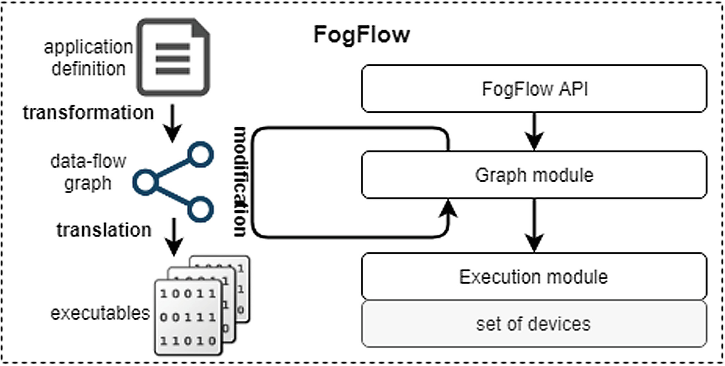
\includegraphics[width=.55\linewidth]{fogflow.png}
\caption[\textit{FogFlow} architecture]{\textit{FogFlow} architecture\cite{fog_flow}.}\label{fig:fogflow}
\end{figure}
    
In a new publication~\cite{fog_flow}, they built the model and engine \textit{FogFlow}, which enables the design of applications able to be decomposed onto heterogeneous IoT environments according to a chosen decomposition schema. To achieve a level of decentralisation and heterogeneity, they abstract out the application definition from its architecture and rely on graph representation to provide an unambiguous, well-defined model of computations. The application definition should be infrastructure-independent and contain only data processing logic, and its execution should be possible on different sets of devices with different capabilities. Several algorithms for flow decomposition are mentioned~\cite{algorithm_fog,ifogsim}, but none were specified in terms of results. \figureref{fig:fogflow} represents the \textit{FogFlow} architecture, which is composed by three modules: (1)~the \textit{FogFlow} API, which enables the creation of the application definition, (2)~the Graph Module, responsible for processing and transforming the application definition into a data flow graph and finally the (3)~Execution Model, which translates the graph and generates executables ready to be run on the assigned devices.

\subsection{\textit{FogFlow}}\label{sec:decentralized_sota_fogflow}

There is another tool with the same name \textit{FogFlow} but created by Cheng et al.~\cite{fogflow_github}. In the first publication related to this tool~\cite{fog_flow_easy}, the contributions made were the implementation of a standards-based programming model for Fog Computing and scalable context management. The first contribution consists in extending the dataflow programming model with hints to facilitate the development of fog applications. The scalable context management introduces a distributed approach, which allows overcoming the limits in a centralised context, achieving much better performance in terms of throughput, response time and scalability. The \textit{FogFlow} framework focuses in a Smart City Platform use case, separated in three areas: (1)~Service Management, typically hosted in the Cloud, (2)~Data Processing, present in cloud and edge devices and (3)~Context Management, which is separated in a device discovery unit hosted in the Cloud and IoT brokers scattered in Edge and Cloud.

\begin{figure}[h]
\centering
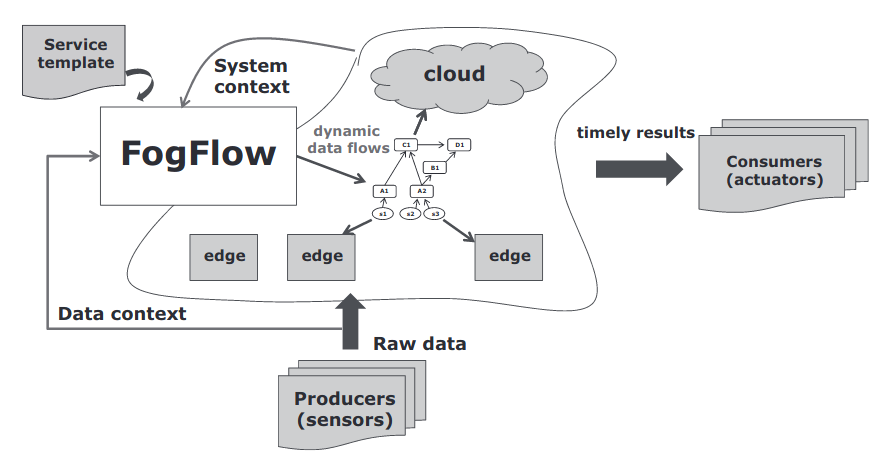
\includegraphics[width=.6\linewidth]{fogflow_tool.png}
\caption[\textit{FogFlow} high level model]{\textit{FogFlow} high level model\cite{fog_flow_tool}.}\label{fig:fogflow_tool}
\end{figure}

In more recent work~\cite{fog_flow_tool}, \textit{FogFlow} was improved to deliver infrastructure providers with an environment that allows them to build decentralised IoT systems faster, with increased stability and scalability. The architecture can be seen in \figureref{fig:fogflow_tool}, where dynamic data representing the IoT system flows that are orchestrated between sensors (Producers) and actuators (Consumers). The application is first designed using the \textit{FogFlow} Task Designer, a hybrid text and visual programming environment, which results in an abstraction called Service Template. This abstraction contains specifics about the resources needed for each part of the system. Once the Service Template is submitted, the framework will determine how to instantiate it using the context data available. Each task is associated with an operator (a Docker image), and its assignment is based on (1)~how many resources are available on each edge node, (2)~the location of data sources, and (3)~the prediction of workload. Edge nodes are autonomous since they can make their own decisions based on their local context, without relying on the central Cloud.

\subsection{DDFlow}\label{sec:decentralized_sota_ddflow}

DDFlow~\cite{ddflow}, first mentioned in \sectionref{sec:slr_results}, presents another distributed approach by extending Node-RED with a system run-time that supports dynamic scaling and adaption of application deployments. The coordinator of the distributed system maintains the state and assigns tasks to available devices, minimizing end-to-end latency. Dataflow notions of \textit{node} and \textit{wire} are expanded, with a \textit{node} in DDFlow representing an instantiation of a task that is deployed in a device, receiving inputs and generating outputs. \textit{Nodes} can be constrained in their assignment by optional parameters, \textit{Device}, and \textit{Region}, inserted by the developer. A \textit{wire} connects two or more nodes and can have three types: \textit{Stream} (one-to-one), \textit{Broadcast} (one-to-many) and \textit{Unite} (many-to-one). 

\begin{figure}[h]
\centering
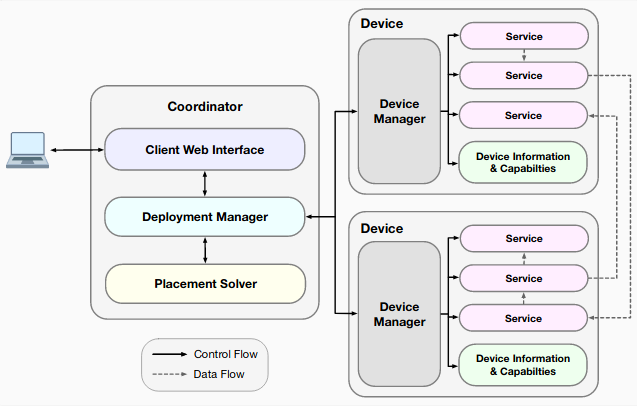
\includegraphics[width=.6\linewidth]{ddflow.png}
\caption[DDFlow architecture]{DDFlow architecture~\cite{ddflow}.}\label{fig:ddflow}
\end{figure}

In a DDFlow system, each device has a set of capabilities and a list of services that correspond to an implementation of a \textit{Node} \seefigureref{fig:ddflow}. The devices communicate this information through their Device Manager or a proxy if it is a constrained device. The coordinator is a web server responsible for managing the DDFlow applications and is composed of three parts, which can be seen in \figureref{fig:ddflow}: (1)~a visual programming environment were DDFlow application are built, (2)~a Deployment Manager that communicates with the Device Managers of the devices and (3)~a Placement Solver, responsible for decomposing and assigning tasks to the available devices. When an application is deployed, a network topology graph and a task graph are constructed based on the real-time information retrieved from the devices. The coordinator proceeds with mapping tasks to devices by minimizing the task graph's end-to-end latency of the longest path. Dynamic adaptation is supported by monitoring the system and adapting to changes. If changes in the network are detected, such as the failure or disconnection of a device, adjustments in the assignment of tasks are made. In addition to this, the coordinator can be replicated onto many devices to improve the reliability and fault-tolerance of the system.

In the evaluation made to DDFlow, the system can recover from network degradation or device overload, whereas in a centralised system, this would cause its total failure.

\subsection{Analysis}\label{sec:decentralized_sota_analysis}

The mentioned tools were characterized based on their mentions or support for the following features and characteristics:

\begin{enumerate}
    \item\textbf{Leverage devices.} A decentralised architecture takes advantage of the computational power of the devices in the network, assigning them tasks. However, some tools can have limitations on the type of devices, making constraints or only focusing on the devices of the Fog tier and not Edge.
    \item\textbf{Capabilities communication.} The devices need to communicate to the orchestrator their capabilities so that it can make an informed decision regarding the decomposition and assignment of tasks.
    \item\textbf{Open-source.} The license of software or tool is essential in terms of its usability. Open-source allows access to the code, making it possible for its analysis, improvement, and reuse.
    \item\textbf{Computation decomposition.} To implement a decentralised architecture, it is important to decompose the computation of the system into independent and logical tasks that can be assigned to devices. This is made using algorithms, which can be specified or mentioned.
    \item\textbf{Run-time adaptation.} A system needs to adapt to run-time changes, such as non-availability of devices or even network failure. The system notices these events and can take action to circumvent the problems and keep functioning.
\end{enumerate}

\begin{table*}[!h]
    \centering
    \label{tab:decentralized_sota_results}
    \begin{threeparttable}
    \resizebox{\textwidth}{!}{
    \begin{tabular}{ l  c  c  c  c  c }
        \toprule
        \textbf{Tool} & \textbf{Leverage devices} & \textbf{Capabilities communication} & \textbf{Open-source} & \textbf{Computation decomposition}  & \textbf{Run-time adaptation}\\
        \midrule
        DDF~\cite{ddf,wotflow_dnr,fog_at_the_edge,exogenous_coordination} & Limited\tnote{1} & \textbullet & \textbullet & Limited\tnote{2} & \textbullet \\
        \textit{FogFlow} \& \textit{uFlow}~\cite{flow_based_programming_fog,fog_flow} & \textbullet & Limited\tnote{3} &  & Limited\tnote{2} & Limited\tnote{3}\\
        \textit{FogFlow}~\cite{fogflow_github,fog_flow_easy,fog_flow_tool} & \textbullet & - & \textbullet & Limited\tnote{2} & \textbullet\\
        \textit{DDFlow}~\cite{ddflow} & Limited\tnote{4} & \textbullet &  & Limited\tnote{2} & \textbullet\\
        \bottomrule
    \end{tabular}
    }
    \caption[Decentralized visual programming solutions applied to IoT and their characteristics.]{Small circles (\textbullet) mean \textit{yes}, hyphens (-) means \textit{no information available}, empty means \textit{no} and asterisk (*) means more than one.}
    \begin{tablenotes}\footnotesize
        \item[1] Assumes that all devices run Node-RED, which limits the type of devices.
        \item[2] Do not specify the algorithm used.
        \item[3] Communication between devices is made through the Cloud.
        \item[4] Assumes that all devices have a list of specific services they can provide.
    \end{tablenotes}
    \end{threeparttable}
\end{table*}

From the analysis and the characteristics of \tableref{tab:decentralized_sota_results}, we can be conclude that the current research in decentralised architectures in visual programming tools applied to IoT is incomplete. All the tools leverage the devices in the network but in different ways. DFF~\cite{ddf} assumes that all devices run Node-RED, which limits the type of devices that can be leveraged since it needs to have minimum resources to run it. \textit{FogFlow} and \textit{uFlow}~\cite{fog_flow,flow_based_programming_fog} is the only tool that specifies how it truly leverages constrained devices, with the transformation of sub-flows into Lua code, with DDFlow~\cite{ddflow} assuming that all devices have a list of specific services they can provide, that should match the node assigned to them.

Regarding the method used to decompose and assign computations to the available devices, DDFlow describes the process with the use of the longest path algorithm focused on reducing end-to-end latency between devices. \textit{FogFlow} and \textit{uFlow}~\cite{fog_flow,flow_based_programming_fog} mention several algorithms that could be used, but do not specify which one was implemented. Both DDF~\cite{ddf} and \textit{FogFlow}~\cite{fog_flow_easy,fog_flow_tool} do not specify the algorithm used besides some constraints but are the only tools with their source code accessible and with an open-source license. All the tools claim to have support for run-time adaptation to changes in the system, such as device failures.

%\cite{mobile_cloud_heterogeneous}
%\cite{mobile_cloud}

\subsection{Conclusion}\label{sec:decentralized_sota_conclusion}

Several solutions are available that provide a decentralized architecture in visual programming tools applied to the Internet-of-Things paradigm. However, some of these tools solve specific problems or make assumptions regarding the scale of the system and the constraints of the devices. We can highlight the following research challenges that remain to be addressed by the research community:

\begin{enumerate}
    \item \textbf{Leveraging devices in the network}: since most tools use a centralized architecture, including Node-RED, they do not leverage the devices in the network. Fog Computing introduces a decentralized solution, one that can be applied to Node-RED by distributing the computational tasks across the edge devices.
    \item \textbf{Communication of computational capabilities}: some of the current tools require the developer to manually introduce the resources of each device in the network, which is not a scalable solution. Others have a specific list of services, manually inserted that the devices can provide. Information about the computational capabilities of the devices in the network is vital for the successful distribution of computation across the devices.
    \item \textbf{Detecting unavailability}: when a device fails or becomes unavailable, the system needs to realize and adapt automatically. The majority of current solutions do not possess this feature, which is vital if a system aims to adapt to changes in the environment dynamically.
    \item \textbf{Code generation of sub-flows}: to truly leverage constrained devices, it is important to convert sub-flows or "tasks" into executable code. Devices that support simple firmware capable of executing code can be used to execute blocks of code, despite their limited capabilities.
    \item \textbf{Provide self-adaption of the system}: devices can fail, as well as the connection between them or even the network. The system needs to discover and identify these changes and adapt to them at run-time in order to keep functioning.
\end{enumerate}

Addressing these research challenges can improve the current state of the Internet-of-Things ecosystem, where systems are mostly centralized, leading to the proliferation of single point of failure (SPOF) (\emph{e.g.}, dependency on the Cloud can render systems unusable if there is an Internet-connectivity problem). Further, high amounts of computational power are unused (\emph{e.g.}, response times could be improved by using on-premises and already existent resources), and can address some pending security and privacy issues~\cite{nocloud}.

We should also mention that although Partha's survey~\cite{survey_vpl_iot} conclude that there exists some advantages of using visual programming languages, such as the ease of visualizing programming logic (which useful for rapid prototyping), and less burden on handling syntax error, as well as mentioning some negative aspects, such as the significant amount of time required for building simple IoT applications, we cannot find support or a rationale on how this observation results from the attributes they analysis (\emph{e.g.}, licence and project repository).


\section{Summary}

\sectionref{sec:slr} presents a Systematic Literature Review of visual programming tools applied to the Internet-of-Things. Each tool derived from the research is summarized and characterized to understand the state of the art regarding this topic of interest. \sectionref{sec:sota_decentralized} describes visual programming tools for building IoT systems that employ a decentralized architecture, pointing out their advantages but also their shortcomings.

